% Options for packages loaded elsewhere
\PassOptionsToPackage{unicode}{hyperref}
\PassOptionsToPackage{hyphens}{url}
\PassOptionsToPackage{dvipsnames,svgnames,x11names}{xcolor}
%
\documentclass[
  10pt,
  a4paper,
]{article}
\usepackage{amsmath,amssymb}
\usepackage{iftex}
\ifPDFTeX
  \usepackage[T1]{fontenc}
  \usepackage[utf8]{inputenc}
  \usepackage{textcomp} % provide euro and other symbols
\else % if luatex or xetex
  \usepackage{unicode-math} % this also loads fontspec
  \defaultfontfeatures{Scale=MatchLowercase}
  \defaultfontfeatures[\rmfamily]{Ligatures=TeX,Scale=1}
\fi
\usepackage{lmodern}
\ifPDFTeX\else
  % xetex/luatex font selection
  \setmainfont[]{Noto Serif CJK SC}
  \setsansfont[]{Noto Sans CJK SC}
  \setmonofont[]{DejaVu Sans Mono}
\fi
% Use upquote if available, for straight quotes in verbatim environments
\IfFileExists{upquote.sty}{\usepackage{upquote}}{}
\IfFileExists{microtype.sty}{% use microtype if available
  \usepackage[]{microtype}
  \UseMicrotypeSet[protrusion]{basicmath} % disable protrusion for tt fonts
}{}
\makeatletter
\@ifundefined{KOMAClassName}{% if non-KOMA class
  \IfFileExists{parskip.sty}{%
    \usepackage{parskip}
  }{% else
    \setlength{\parindent}{0pt}
    \setlength{\parskip}{6pt plus 2pt minus 1pt}}
}{% if KOMA class
  \KOMAoptions{parskip=half}}
\makeatother
\usepackage{xcolor}
\usepackage[margin=20mm]{geometry}
\usepackage{color}
\usepackage{fancyvrb}
\newcommand{\VerbBar}{|}
\newcommand{\VERB}{\Verb[commandchars=\\\{\}]}
\DefineVerbatimEnvironment{Highlighting}{Verbatim}{commandchars=\\\{\}}
% Add ',fontsize=\small' for more characters per line
\newenvironment{Shaded}{}{}
\newcommand{\AlertTok}[1]{\textcolor[rgb]{1.00,0.00,0.00}{\textbf{#1}}}
\newcommand{\AnnotationTok}[1]{\textcolor[rgb]{0.38,0.63,0.69}{\textbf{\textit{#1}}}}
\newcommand{\AttributeTok}[1]{\textcolor[rgb]{0.49,0.56,0.16}{#1}}
\newcommand{\BaseNTok}[1]{\textcolor[rgb]{0.25,0.63,0.44}{#1}}
\newcommand{\BuiltInTok}[1]{\textcolor[rgb]{0.00,0.50,0.00}{#1}}
\newcommand{\CharTok}[1]{\textcolor[rgb]{0.25,0.44,0.63}{#1}}
\newcommand{\CommentTok}[1]{\textcolor[rgb]{0.38,0.63,0.69}{\textit{#1}}}
\newcommand{\CommentVarTok}[1]{\textcolor[rgb]{0.38,0.63,0.69}{\textbf{\textit{#1}}}}
\newcommand{\ConstantTok}[1]{\textcolor[rgb]{0.53,0.00,0.00}{#1}}
\newcommand{\ControlFlowTok}[1]{\textcolor[rgb]{0.00,0.44,0.13}{\textbf{#1}}}
\newcommand{\DataTypeTok}[1]{\textcolor[rgb]{0.56,0.13,0.00}{#1}}
\newcommand{\DecValTok}[1]{\textcolor[rgb]{0.25,0.63,0.44}{#1}}
\newcommand{\DocumentationTok}[1]{\textcolor[rgb]{0.73,0.13,0.13}{\textit{#1}}}
\newcommand{\ErrorTok}[1]{\textcolor[rgb]{1.00,0.00,0.00}{\textbf{#1}}}
\newcommand{\ExtensionTok}[1]{#1}
\newcommand{\FloatTok}[1]{\textcolor[rgb]{0.25,0.63,0.44}{#1}}
\newcommand{\FunctionTok}[1]{\textcolor[rgb]{0.02,0.16,0.49}{#1}}
\newcommand{\ImportTok}[1]{\textcolor[rgb]{0.00,0.50,0.00}{\textbf{#1}}}
\newcommand{\InformationTok}[1]{\textcolor[rgb]{0.38,0.63,0.69}{\textbf{\textit{#1}}}}
\newcommand{\KeywordTok}[1]{\textcolor[rgb]{0.00,0.44,0.13}{\textbf{#1}}}
\newcommand{\NormalTok}[1]{#1}
\newcommand{\OperatorTok}[1]{\textcolor[rgb]{0.40,0.40,0.40}{#1}}
\newcommand{\OtherTok}[1]{\textcolor[rgb]{0.00,0.44,0.13}{#1}}
\newcommand{\PreprocessorTok}[1]{\textcolor[rgb]{0.74,0.48,0.00}{#1}}
\newcommand{\RegionMarkerTok}[1]{#1}
\newcommand{\SpecialCharTok}[1]{\textcolor[rgb]{0.25,0.44,0.63}{#1}}
\newcommand{\SpecialStringTok}[1]{\textcolor[rgb]{0.73,0.40,0.53}{#1}}
\newcommand{\StringTok}[1]{\textcolor[rgb]{0.25,0.44,0.63}{#1}}
\newcommand{\VariableTok}[1]{\textcolor[rgb]{0.10,0.09,0.49}{#1}}
\newcommand{\VerbatimStringTok}[1]{\textcolor[rgb]{0.25,0.44,0.63}{#1}}
\newcommand{\WarningTok}[1]{\textcolor[rgb]{0.38,0.63,0.69}{\textbf{\textit{#1}}}}
\usepackage{longtable,booktabs,array}
\usepackage{calc} % for calculating minipage widths
% Correct order of tables after \paragraph or \subparagraph
\usepackage{etoolbox}
\makeatletter
\patchcmd\longtable{\par}{\if@noskipsec\mbox{}\fi\par}{}{}
\makeatother
% Allow footnotes in longtable head/foot
\IfFileExists{footnotehyper.sty}{\usepackage{footnotehyper}}{\usepackage{footnote}}
\makesavenoteenv{longtable}
\usepackage{graphicx}
\makeatletter
\def\maxwidth{\ifdim\Gin@nat@width>\linewidth\linewidth\else\Gin@nat@width\fi}
\def\maxheight{\ifdim\Gin@nat@height>\textheight\textheight\else\Gin@nat@height\fi}
\makeatother
% Scale images if necessary, so that they will not overflow the page
% margins by default, and it is still possible to overwrite the defaults
% using explicit options in \includegraphics[width, height, ...]{}
\setkeys{Gin}{width=\maxwidth,height=\maxheight,keepaspectratio}
% Set default figure placement to htbp
\makeatletter
\def\fps@figure{htbp}
\makeatother
\setlength{\emergencystretch}{3em} % prevent overfull lines
\providecommand{\tightlist}{%
  \setlength{\itemsep}{0pt}\setlength{\parskip}{0pt}}
\setcounter{secnumdepth}{-\maxdimen} % remove section numbering
\ifLuaTeX
\usepackage[bidi=basic]{babel}
\else
\usepackage[bidi=default]{babel}
\fi
\babelprovide[main,import]{chinese}
\ifPDFTeX
\else
\babelfont{rm}[]{Noto Serif CJK SC}
\fi
% get rid of language-specific shorthands (see #6817):
\let\LanguageShortHands\languageshorthands
\def\languageshorthands#1{}
\usepackage{xurl}
\usepackage{tikz}
\usetikzlibrary{arrows.meta,positioning}
\usepackage{fancyhdr}
\XeTeXlinebreaklocale "zh"
\XeTeXlinebreakskip=0pt plus 1pt
\setlength{\emergencystretch}{3em}
\setlength{\headheight}{15pt}
\pagestyle{fancy}
\fancyhf{}
\fancyhead[L]{\small diffuse-mixing / LTN}
\fancyhead[R]{\small 理论、代码与证据总报告}
\fancyfoot[C]{\thepage}
\AtBeginDocument{\hypersetup{pdfauthor={diffuse-mixing research project},pdftitle={LTN 扩散与掺混：理论、代码、证据与下一步}}}
\ifLuaTeX
  \usepackage{selnolig}  % disable illegal ligatures
\fi
\usepackage{bookmark}
\IfFileExists{xurl.sty}{\usepackage{xurl}}{} % add URL line breaks if available
\urlstyle{same}
\hypersetup{
  pdftitle={LTN 扩散与掺混},
  pdfauthor={diffuse-mixing 项目整理},
  pdflang={zh-CN},
  colorlinks=true,
  linkcolor={blue},
  filecolor={Maroon},
  citecolor={Blue},
  urlcolor={blue},
  pdfcreator={LaTeX via pandoc}}

\title{LTN 扩散与掺混}
\usepackage{etoolbox}
\makeatletter
\providecommand{\subtitle}[1]{% add subtitle to \maketitle
  \apptocmd{\@title}{\par {\large #1 \par}}{}{}
}
\makeatother
\subtitle{理论主线、代码实现、验证证据与下一步工作}
\author{diffuse-mixing 项目整理}
\date{2026-11-07}

\begin{document}
\maketitle

\renewcommand*\contentsname{目录}
{
\hypersetup{linkcolor=}
\setcounter{tocdepth}{2}
\tableofcontents
}
本报告整理现有研究，不新增物理实验。Stage3 尚未通过，fluid ORC 关闭。 旧
v0.8.0 未恢复；当前软件检查、限定算例结果和一般物理主张分别说明。
用户已要求更新 GitHub；远端是否完成以交接回执为准。

\newpage

\section{LTN
扩散与掺混：理论主线、实现与验证总览}\label{ltn-ux6269ux6563ux4e0eux63baux6df7ux7406ux8bbaux4e3bux7ebfux5b9eux73b0ux4e0eux9a8cux8bc1ux603bux89c8}

整理日期：2026-11-07。依据本地恢复点 \nolinkurl{f4a6822}
及其保存结果。本文是当前阅读入口；原规范和历史结果保持原样。

\textbf{项目承接了原理论的质量测度、局部交换和时序传播主线，已经完成图层实现及多组限定流动的验证；``由轨迹可靠预测一般流体掺混，再解释动态
ORC''的完整方法仍未验收。Stage3 为 incomplete，fluid ORC
关闭。按用户要求暂停新增研究，本次只整理文档。}

\subsection{1.
最初要解决什么，现在走到哪里}\label{ux6700ux521dux8981ux89e3ux51b3ux4ec0ux4e48ux73b0ux5728ux8d70ux5230ux54eaux91cc}

原目标是：从带有固定身份的流体轨迹、初始质量和扩散本构出发，描述哪些物质发生交换、给定浓度场如何均匀化，再用动态曲率描述传播的收缩性质。位置靠近、界面拉长或网络结构变化，本身不等于分子混合。

\begin{center}
\begin{tikzpicture}[box/.style={draw,rounded corners,align=center,text width=36mm,minimum height=12mm,font=\small},>=Stealth]
\node[box] (a) {轨迹身份\\固定物质质量};
\node[box,right=8mm of a] (b) {当前邻接\\物理交换导通率};
\node[box,right=8mm of b] (c) {按时间顺序\\传播浓度};
\node[box,below=12mm of a] (f) {参考物质图\\固定距离};
\node[box,below=12mm of b] (d) {实际初场的\\掺混与耗散};
\node[box,below=12mm of c] (e) {动态 ORC\\流体解释未启用};
\draw[->] (a)--(b);\draw[->] (b)--(c);
\draw[->] (a)--(f);\draw[->] (c)--(d);\draw[->] (c)--(e);
\draw[->] (f.south)--++(0,-5mm)-|(e.south);
\node[above=4mm of b,font=\small] (g) {密度来源与扩散本构};
\draw[->] (g)--(b);
\end{tikzpicture}
\end{center}

当前最主要的科学问题仍在第二个框：\textbf{什么局部交换规则既保持质量、正性，又准确逼近目标扩散方程？}
后面的传播和统计不能弥补这里的物理误差。

前期先用真实物质面建立普通有限体积基线，回答``质量平均未知量应该怎样交换''；随后转向从轨迹点、密度和边界构造交换面的候选，回答``如何接回
LTN 的输入''。最近的 kernel/ledger
研究检查的是上图中``密度来源''这个输入环节。它有必要，但不能代替整条理论主线。

此前按轮次不断拆分诊断、契约和审计，使局部问题占据了交接首页。这次改为按理论环节阅读；126
条历史记录只作追溯，不作为理解项目的先决条件。

\subsection{2.
与最初理论各部分的关系}\label{ux4e0eux6700ux521dux7406ux8bbaux5404ux90e8ux5206ux7684ux5173ux7cfb}

这里以原始
\href{https://github.com/hongjianli97/diffuse-mixing/blob/main/docs/METHOD.md}{\nolinkurl{METHOD.md}}
的最终约定为主，结合
\href{https://github.com/hongjianli97/diffuse-mixing/blob/main/docs/CODE_REVIEW.md}{\nolinkurl{CODE_REVIEW.md}}
对旧
LHD/原型代码的审查。早期报告中的其他理论分支仍保留，不把它们都算成本阶段已经实现的内容。

\begin{longtable}[]{@{}
  >{\raggedright\arraybackslash}p{(\columnwidth - 4\tabcolsep) * \real{0.3333}}
  >{\raggedright\arraybackslash}p{(\columnwidth - 4\tabcolsep) * \real{0.3333}}
  >{\raggedright\arraybackslash}p{(\columnwidth - 4\tabcolsep) * \real{0.3333}}@{}}
\toprule\noalign{}
\begin{minipage}[b]{\linewidth}\raggedright
原有思想或成果
\end{minipage} & \begin{minipage}[b]{\linewidth}\raggedright
在当前工作的具体位置
\end{minipage} & \begin{minipage}[b]{\linewidth}\raggedright
当前能够支持的说法
\end{minipage} \\
\midrule\noalign{}
\endhead
\bottomrule\noalign{}
\endlastfoot
拉格朗日轨迹网络 LTN & 固定物质身份；参考邻接与当前交换邻接分开 &
延续原主线；轨迹还需质量、密度来源、D 和边界信息才能确定扩散问题 \\
LHD 中的质量测度与密度账本 & 固定质量矩阵 M；oracle、核重构、固定邻居环
ledger 分别作为密度来源 & 继承质量测度思想；当前无 F
拟合的环代理不等于旧 ledger\_v4，也不代表完整 LHD 已移植 \\
界面拉伸、压缩与掺混 & 解释流动如何改变物质接近、方向和扩散距离 &
在光滑、薄层等适用条件下作为解释与对照；拉伸率不直接充当全局混合率 \\
网络扩散 & 对称非负导通率、固定质量生成元、时间有序传播 &
图层性质明确；流体连续一致性必须另验 \\
AFRC 与动态 ORC & AFRC 保留结构识别定位；ORC 对传播核及参考距离定义收缩
& 两者不等价；目前没有流体 ORC 的新计算结论 \\
Hodge/Dirac、压力、黏性功、声学等 & 原始资料和理论背景 & 按原 METHOD 第
10 节不进入本篇扩散掺混主线；本阶段不宣称验证这些分支 \\
\end{longtable}

当前工作是在验证原理论中``运动学信息怎样变成可信物理交换''的关键环节。它尚未完成原理论的全部应用，也没有以有限体积本身取代
LTN 目标。

\subsection{3.
需要固定下来的数学对象}\label{ux9700ux8981ux56faux5b9aux4e0bux6765ux7684ux6570ux5b66ux5bf9ux8c61}

\subsubsection{物质状态与密度语义}\label{ux7269ux8d28ux72b6ux6001ux4e0eux5bc6ux5ea6ux8bedux4e49}

物质单元随流运动，质量固定，状态为质量平均：

\[
m_i=\int_{K_i(t)}\rho\,dV,\qquad
\bar c_i=\frac{1}{m_i}\int_{K_i(t)}\rho c\,dV.
\]

轨迹点浓度、点密度 \(\rho(X_i,t)\)、物质单元平均密度 \(m_i/|K_i(t)|\)
是不同对象。辅助 Voronoi
面可用于构造候选交换，但其区域不是自动随流运动的真实物质单元；也不能据此把质量改为``点密度
× 当前 Voronoi 面积''。在核求积中，\(m_i/\rho(X_i,t)\)
只是相应求积权重，不天然等于真实物质体积。

\subsubsection{两套基础图与派生传播核}\label{ux4e24ux5957ux57faux7840ux56feux4e0eux6d3eux751fux4f20ux64adux6838}

\begin{itemize}
\tightlist
\item
  参考物质图 \(G_{ref}\)：固定标签和参考边长，形成 ORC 使用的距离
  \(d_0\)。
\item
  当前交换图 \(G_{ex}(t)\)：同一批标签，当前局部邻接和导通率
  \(g_{ij}(t)\)。
\item
  传播核 \(P(t_1,t_0)\)：由交换演化得到，不是额外任意指定的一套基础图。
\end{itemize}

令
\(M=\operatorname{diag}(m_i)\)、\(L=B^T\operatorname{diag}(g)B\)，图层方程为

\[
M\dot{\bar c}+L(t)\bar c=0,\qquad Q=-M^{-1}L.
\]

固定正质量、对称非负导通率和封闭边界给出质量守恒、常数保持、最大值原理和方差耗散。这些是有条件的离散代数性质。还需证明或数值验证该离散逼近
\(\rho D_t c=\nabla\cdot(\rho D\nabla c)\)，才可以作相应流体解释。\(\Gamma=\rho D\)，恒
D 与恒 Γ 是不同本构，不能混为同一个精度比较。

传播必须保持时间顺序。原规范默认隐式
Euler：\(A_n=(M+\Delta t_n L_n)^{-1}M\)，\(P=A_{K-1}\cdots A_0\)。一般不能用平均生成元的一次指数替代这个过程。当前部分研究用冻结中点指数作用，并以独立
uniformization 递推核验；其验证不能直接算作默认隐式 Euler
生产接口已完成迁移。

\subsubsection{实际掺混与曲率分别回答什么}\label{ux5b9eux9645ux63baux6df7ux4e0eux66f2ux7387ux5206ux522bux56deux7b54ux4ec0ux4e48}

设 \(c_m=\sum_i m_i\bar c_i/\sum_i m_i\)，

\[
E=\tfrac12\sum_i m_i(\bar c_i-c_m)^2,\quad
\chi=\sum_{i<j}g_{ij}(\bar c_i-\bar c_j)^2,\quad
\dot E=-\chi,\quad H=1-E(t)/E(0).
\]

\(H\) 描述给定初场的质量方差减少，\(E(0)=0\)
单独处理。时间离散造成的附加耗散须与上述半离散交换耗散分开。当前
\nolinkurl{voronoi_time_action.metrics} 的 \nolinkurl{variance} 字段保存
\(\sum m_i(\bar c_i-c_m)^2=2E\)，其比值 H
与这里一致；读取绝对耗散量时须保留这个因子约定。

动态 ORC 的约定为

\[
\kappa_{ij}=1-\frac{W_{1,d_0}(P_{i,:},P_{j,:})}{d_0(i,j)}.
\]

该定义只用于 \(0<d_0(i,j)<\infty\)
的探针对。它描述指定度量与时间窗下的最坏 Lipschitz
对比收缩，不能代替某个实际初场的 \(H\)。\(D=0\)
应给出恒等传播和无扩散掺混；压缩且 \(D>0\) 则可能增强扩散。当前
\(\kappa\) 未计算，fluid ORC 继续关闭。

\subsection{4.
理论对象对应哪些代码}\label{ux7406ux8bbaux5bf9ux8c61ux5bf9ux5e94ux54eaux4e9bux4ee3ux7801}

当前可读取的新增实现主要位于 \nolinkurl{research/}。原
\href{https://github.com/hongjianli97/diffuse-mixing/blob/main/docs/CODEX_TASK.md}{\nolinkurl{CODEX_TASK.md}}
所列 \nolinkurl{src/ltnmix/}、CLI
和打包接口是设计任务，不能用那份清单声称当前已有完整产品。旧 v0.8.0、246
项测试及其目标 NPZ 尚未恢复。

\begin{longtable}[]{@{}
  >{\raggedright\arraybackslash}p{(\columnwidth - 4\tabcolsep) * \real{0.3333}}
  >{\raggedright\arraybackslash}p{(\columnwidth - 4\tabcolsep) * \real{0.3333}}
  >{\raggedright\arraybackslash}p{(\columnwidth - 4\tabcolsep) * \real{0.3333}}@{}}
\toprule\noalign{}
\begin{minipage}[b]{\linewidth}\raggedright
环节
\end{minipage} & \begin{minipage}[b]{\linewidth}\raggedright
实际代码入口
\end{minipage} & \begin{minipage}[b]{\linewidth}\raggedright
用途及边界
\end{minipage} \\
\midrule\noalign{}
\endhead
\bottomrule\noalign{}
\endlastfoot
固定身份、质量、两图及小图传播 &
\href{https://github.com/hongjianli97/diffuse-mixing/blob/main/research/reconnect/trajectory_chain.py}{\nolinkurl{trajectory_chain.py}}
&
\nolinkurl{TrajectorySamples}、\nolinkurl{laplacian}、\nolinkurl{reference_distances}、\nolinkurl{propagate_supplied}；调用方提供电导，不能自动保证流体一致性 \\
真实物质面普通中心阻力基线 &
\href{https://github.com/hongjianli97/diffuse-mixing/blob/main/research/material_fv/material_fv.py}{\nolinkurl{material_fv.py}}
& 一维真实移动面；几何中点间积分阻力、固定质量、隐式 Euler \\
Becker 重建与三种通量对照 &
\href{https://github.com/hongjianli97/diffuse-mixing/blob/main/research/rebuild/experiment.py}{\nolinkurl{experiment.py}}、\href{https://github.com/hongjianli97/diffuse-mixing/blob/main/research/rebuild/reference.py}{\nolinkurl{reference.py}}
&
几何中点、质量中点、质量平均阻力明确分列；独立细网格参考及物质平均投影 \\
轨迹点生成候选交换面 &
\href{https://github.com/hongjianli97/diffuse-mixing/blob/main/research/reconnect/periodic_voronoi_fv.py}{\nolinkurl{periodic_voronoi_fv.py}}、\href{https://github.com/hongjianli97/diffuse-mixing/blob/main/research/reconnect/bounded_periodic_voronoi.py}{\nolinkurl{bounded_periodic_voronoi.py}}
&
普通串联阻力候选；周期和有界几何各有适用条件，辅助面不被冒称为真实物质面 \\
稀疏作用、独立递推与掺混量 &
\href{https://github.com/hongjianli97/diffuse-mixing/blob/main/research/reconnect/voronoi_time_action.py}{\nolinkurl{voronoi_time_action.py}}
&
\nolinkurl{operators}、\nolinkurl{exponential}、\nolinkurl{uniformization}、\nolinkurl{metrics}、\nolinkurl{dissipation}；研究级推进与核验 \\
密度适配 &
\href{https://github.com/hongjianli97/diffuse-mixing/blob/main/research/reconnect/t1_density_sources.py}{\nolinkurl{t1_density_sources.py}}、\href{https://github.com/hongjianli97/diffuse-mixing/blob/main/research/reconnect/compression_density_sources.py}{\nolinkurl{compression_density_sources.py}}
& 固定质量核重构和固定邻居环代理；与 oracle 使用同一后端比较 \\
平滑流及接触参考 &
\href{https://github.com/hongjianli97/diffuse-mixing/blob/main/research/reconnect/compression_reference.py}{\nolinkurl{compression_reference.py}}、\href{https://github.com/hongjianli97/diffuse-mixing/blob/main/research/reconnect/contact_spectral_reference.py}{\nolinkurl{contact_spectral_reference.py}}
& 独立参考与误差控制；不是用候选结果反拟合参考 \\
动态 ORC & 原 METHOD 第 8
节；\href{https://github.com/hongjianli97/diffuse-mixing/blob/main/research/reconnect/MAINLINE_RECONNECTION.md}{主线回接报告}
& 保留定义与启用条件；当前重建链没有已验收的流体 ORC 实现成果 \\
\end{longtable}

\nolinkurl{reference_baseline/}、\nolinkurl{prototypes/}、\nolinkurl{legacy_sources/}
是保留的历史来源。代码中旧的裁剪、补质量和 F
拟合分支，不因被保留而成为当前允许的默认路径。

\subsection{5.
哪些验证已经有了}\label{ux54eaux4e9bux9a8cux8bc1ux5df2ux7ecfux6709ux4e86}

下表是保存结果的归纳，未在此次整理中重跑。详细来源见
\href{https://github.com/hongjianli97/diffuse-mixing/blob/main/research/reconnect/JOINT_EVIDENCE_REVIEW.md}{联合证据报告}
和
\href{https://github.com/hongjianli97/diffuse-mixing/blob/main/runs/reconnect-joint-evidence/evidence-ledger.json}{逐条证据账本}。T0--T6
是实验编号，与实施阶段 Stage1--Stage4 不同，T3 通过不等于 Stage3 通过。

\begin{longtable}[]{@{}
  >{\raggedright\arraybackslash}p{(\columnwidth - 4\tabcolsep) * \real{0.3333}}
  >{\raggedright\arraybackslash}p{(\columnwidth - 4\tabcolsep) * \real{0.3333}}
  >{\raggedright\arraybackslash}p{(\columnwidth - 4\tabcolsep) * \real{0.3333}}@{}}
\toprule\noalign{}
\begin{minipage}[b]{\linewidth}\raggedright
层级或算例
\end{minipage} & \begin{minipage}[b]{\linewidth}\raggedright
已有证据
\end{minipage} & \begin{minipage}[b]{\linewidth}\raggedright
仍需遵守的范围
\end{minipage} \\
\midrule\noalign{}
\endhead
\bottomrule\noalign{}
\endlastfoot
离散图层 &
小图质量、正性、能量、传播方向和时间非对易检查；\href{https://github.com/hongjianli97/diffuse-mixing/blob/main/research/reconnect/MAINLINE_RECONNECTION.md}{主线回接}
& 给定图的正确性不证明电导代表真实流体 \\
真物质面 Becker 基线 & 三种通量、时间/参考检查及 32/64/128
列空间细化；\href{https://github.com/hongjianli97/diffuse-mixing/blob/main/research/rebuild/SPATIAL_CONVERGENCE.md}{空间报告}
& 固定物理问题的观察阶接近二阶；不等于通用点轨迹后端验收 \\
T1 静止正弦 & oracle
三空间档与时间控制；\href{https://github.com/hongjianli97/diffuse-mixing/blob/main/research/reconnect/T1_UNIFORM_COMPARISON.md}{T1
报告} & 限定均匀周期物质平均案例 \\
T2 客观性、零扩散 &
\href{https://github.com/hongjianli97/diffuse-mixing/blob/main/research/reconnect/T2_TRANSLATION_COMPARISON.md}{平移}、\href{https://github.com/hongjianli97/diffuse-mixing/blob/main/research/reconnect/T2_D0_COMPARISON.md}{D=0}、\href{https://github.com/hongjianli97/diffuse-mixing/blob/main/research/reconnect/T2_ROTATION_COMPARISON.md}{共转边界}
控制 & 限定输入和边界；没有运行曲率 \\
T3 平滑运动 &
\href{https://github.com/hongjianli97/diffuse-mixing/blob/main/research/reconnect/T3_AFFINE_SPATIAL_COMPARISON.md}{仿射压缩}、\href{https://github.com/hongjianli97/diffuse-mixing/blob/main/research/reconnect/AFFINE_SHEAR_SPATIAL_COMPARISON.md}{仿射剪切}
三档及本构/方向控制；非线性周期压缩 oracle 空间证据 & 原 N32
未决记录保留；不能外推任意平滑流动或所有密度来源 \\
T4 独立接触 &
\href{https://github.com/hongjianli97/diffuse-mixing/blob/main/research/reconnect/CONTACT_SPATIAL_COMPARISON.md}{静态接触
oracle 三档} & 不代替移动激波和三来源比较 \\
T4 移动 Becker & δ=.08、共同 K32、32/64/128
列的八项空间改善分辨；\href{https://github.com/hongjianli97/diffuse-mixing/blob/main/research/reconnect/BECKER_COMMON_K32_COMPARISON.md}{共同
K32 报告} & 固定八行的一维列细化；旧 K16 空间及后移 H 时间未决保持 \\
层厚度变化 &
\href{https://github.com/hongjianli97/diffuse-mixing/blob/main/research/reconnect/BECKER_DELTA004_COMPARISON.md}{δ=.04
固定物质质量对照} 已执行 & 该例状态时间控制分辨，H 时间未分辨；只有
N32，两厚度不构成 δ→0 极限 \\
同后端密度来源 & T1 N32、平滑运动 N64
的来源对照；\href{https://github.com/hongjianli97/diffuse-mixing/blob/main/research/reconnect/COMPRESSION_JOINT_CONTROL_RESULTS.md}{联合时间/参考控制}
& 已有单例，不等于瞬态三来源空间与接触/激波覆盖完成 \\
\end{longtable}

\subsubsection{最初 FV
判别实验的真实结果}\label{ux6700ux521d-fv-ux5224ux522bux5b9eux9a8cux7684ux771fux5b9eux7ed3ux679c}

旧独立原型所报 \nolinkurl{4.2237e-4}、\nolinkurl{4.9382e-4} 和旧核结果
\nolinkurl{1.7642e-3} 没有原 NPZ 可核对，不作为本仓库已复现的测量值。

独立重建的同一 Becker 参数 δ=.08、D=.02、T=.1、32 个物质列，512
步结果为：

\begin{longtable}[]{@{}lr@{}}
\toprule\noalign{}
当前重建定义 & 相对初始质量波动范数的浓度误差 \\
\midrule\noalign{}
\endhead
\bottomrule\noalign{}
\endlastfoot
普通阻力，真实单元几何中点 & 5.69194e-4 \\
普通阻力，质量区间中点映射到空间 & 4.36001e-4 \\
质量平均阻力通量 & 5.12753e-4 \\
\end{longtable}

来源：\href{https://github.com/hongjianli97/diffuse-mixing/blob/main/research/rebuild/REPORT.md}{重建报告}。中心约定会改变排序；常通量精确不能保证瞬态最优。普通几何中点保持原定基线，其余作为对照，不能按误差最小者悄悄更名。上述数据不能证明相对丢失旧核结果的改善倍数。

\subsubsection{最近的密度研究到底说明什么}\label{ux6700ux8fd1ux7684ux5bc6ux5ea6ux7814ux7a76ux5230ux5e95ux8bf4ux660eux4ec0ux4e48}

在同一平滑压缩的一个保存时刻，固定
\nolinkurl{h=2/N}，N=64/128/256：kernel 点密度相对质量 L² 误差约
\nolinkurl{6.17e-4 → 6.38e-4 → 6.44e-4}；固定环 ledger 约
\nolinkurl{2.85e-4 → 7.14e-5 → 1.78e-5}。这是\href{https://github.com/hongjianli97/diffuse-mixing/blob/main/research/reconnect/DENSITY_SNAPSHOT_COMPARISON.md}{单快照密度对照}，没有在这些新密度场上运行新的标量传播。

随后\href{https://github.com/hongjianli97/diffuse-mixing/blob/main/research/reconnect/DENSITY_ERROR_STRUCTURE.md}{误差结构复核}和\href{https://github.com/hongjianli97/diffuse-mixing/blob/main/research/reconnect/DENSITY_KERNEL_CONSISTENCY.md}{一致性推导}解释了固定核宽/粒子间距比例下的求积问题；结论受既定映射、采样和光滑性限制。ledger
的局部结果不能外推激波，kernel 的这一失败也不等于所有核方法失败。

此前出现的``近似密度让浓度误差更小''，包含与交换离散残差的抵消，不能说它比给定密度真值更准确。该分支在总报告中只承担密度输入诊断，不升级为项目新目标。

\subsection{6. Stage3
还差什么，哪些并非新的通过条件}\label{stage3-ux8fd8ux5deeux4ec0ux4e48ux54eaux4e9bux5e76ux975eux65b0ux7684ux901aux8fc7ux6761ux4ef6}

原验收依据是 METHOD 第 11--13 节和 CODEX\_TASK
第三阶段。本次不改变它们、不增设阈值，也不把完成度换算成百分比。

\begin{longtable}[]{@{}
  >{\raggedright\arraybackslash}p{(\columnwidth - 4\tabcolsep) * \real{0.3333}}
  >{\raggedright\arraybackslash}p{(\columnwidth - 4\tabcolsep) * \real{0.3333}}
  >{\raggedright\arraybackslash}p{(\columnwidth - 4\tabcolsep) * \real{0.3333}}@{}}
\toprule\noalign{}
\begin{minipage}[b]{\linewidth}\raggedright
尚未闭合的问题
\end{minipage} & \begin{minipage}[b]{\linewidth}\raggedright
与原要求的关系
\end{minipage} & \begin{minipage}[b]{\linewidth}\raggedright
目前的边界
\end{minipage} \\
\midrule\noalign{}
\endhead
\bottomrule\noalign{}
\endlastfoot
同后端三密度来源的完整物理比较 & CODEX\_TASK 第三阶段、METHOD
密度误差拆分 &
平滑单例和单时刻密度空间证据已经存在；仍缺相应瞬态空间、接触/激波覆盖，失败候选须保留失败及适用限制 \\
激波的空间、时间与层厚度影响分开 & CODEX\_TASK 要求分别控制 h、Δt、δ &
δ=.08 有有效空间证据；δ=.04 只有单档空间且 H
时间未分辨，不能宣布一般层厚度收敛 \\
研究候选的物理适用范围 & METHOD 要求正交换后端完成 T1--T4 后再作流体解释
&
真物质面基线、辅助面候选、不同边界包装器须分别标明；不能拼接局部成功来宣称通用后端通过 \\
\end{longtable}

还要区分以下三类问题：

\begin{itemize}
\tightlist
\item
  \textbf{已登记的诊断未决项}：如部分 Becker 后移 H 检查、N64
  ledger/oracle 终时 H
  改善低于不确定度。保留原判定；不能改阈值制造通过，也不能据此要求无限增加时间档。
\item
  \textbf{不是原验收要求的``胜负''}：ledger 必须胜过
  oracle、每种新通量必须优于普通 FV，都不是 Stage3
  完成条件。准确性、收敛与适用范围才是要回答的问题。
\item
  \textbf{后续应用或交付目标}：复杂二维非平面激波、DNS、T5/T6、完整 ORC
  应用、生产 CLI/包迁移仍有工作，但不一概追加为当前解析 Stage3
  的新前提。旧 v0.8.0 能否找回也不是新研究完成的物理条件。
\end{itemize}

当前累计 \textbf{508 项检查记录}，包含重建软件与研究检查；不是 508
个独立物理算例，不包含尚未恢复的旧 246 项，也不是本轮重新执行 508
项。检查数量不表示 Stage3 完成程度。

\subsection{7.
整理后的阅读方式与后续边界}\label{ux6574ux7406ux540eux7684ux9605ux8bfbux65b9ux5f0fux4e0eux540eux7eedux8fb9ux754c}

\begin{enumerate}
\def\labelenumi{\arabic{enumi}.}
\tightlist
\item
  理解项目：读本文。
\item
  核对原定义：读
  \href{https://github.com/hongjianli97/diffuse-mixing/blob/main/docs/METHOD.md}{\nolinkurl{METHOD.md}}
  和
  \href{https://github.com/hongjianli97/diffuse-mixing/blob/main/docs/CODEX_TASK.md}{\nolinkurl{CODEX_TASK.md}}。它们保持原始字节，不追写新状态。
\item
  查某项证据：从第 5 节进入对应报告，再查 \nolinkurl{runs/}
  的结果、输入和哈希；具体时间、边界、中心与误差定义以该报告为准。
\item
  查全过程：\href{https://github.com/hongjianli97/diffuse-mixing/blob/main/docs/RESEARCH_STATUS.md}{\nolinkurl{RESEARCH_STATUS.md}}
  保留追加式历史索引；旧 PHASE 文档是有日期的快照。
\item
  新聊天交接或恢复：从
  \href{https://github.com/hongjianli97/diffuse-mixing/blob/main/GITHUB_HANDOFF.md}{\nolinkurl{GITHUB_HANDOFF.md}}
  开始，按备份清单核验实际可恢复范围。
\end{enumerate}

\textbf{当前执行状态是研究暂停、文档整理完成。}
\nolinkurl{runs/reconnect-density-error-structure/next-gate-spec.json}
中固定旧带宽求积对照仅保留为历史建议，不再是自动执行的下一步。它及旧报告中的``下一步''均不能覆盖用户现在暂停研究的要求。

恢复研究时，应先明确要检验的具体主张及最小判别证据，再落实单个问题；每次进展说明都回到``原理论哪一环、得到什么证据、还不能说明什么''。不以增加报告、审计次数或反复加密代替物理结论。总览初次整理未运行新算例、未修改数值代码或旧结果。后续经用户要求制作完整
PDF、整理代码并更新 GitHub，见
\href{https://github.com/hongjianli97/diffuse-mixing/blob/main/docs/CODE_GUIDE.md}{代码指南}、\href{https://github.com/hongjianli97/diffuse-mixing/blob/main/docs/NEXT_STEPS.md}{下一步计划}
和当前交接入口；新物理实验仍未执行。

\newpage

\section{理论与数值证据附录}\label{ux7406ux8bbaux4e0eux6570ux503cux8bc1ux636eux9644ux5f55}

本附录重述已有规范及重建推导，不提出新的模型假设，不重算保存数据。

\subsection{从连续方程到物质平均交换}\label{ux4eceux8fdeux7eedux65b9ux7a0bux5230ux7269ux8d28ux5e73ux5747ux4ea4ux6362}

连续性和被动质量分数方程为

\[
\partial_t\rho+\nabla\cdot(\rho u)=0,\qquad
\partial_t(\rho c)+\nabla\cdot(\rho u c)=\nabla\cdot(\rho D\nabla c).
\]

对随流运动的物质区域应用输运定理，对流通量被物质边界运动抵消：

\[
\dot m_i=0,\qquad
m_i\dot{\bar c}_i=\int_{\partial K_i(t)}\rho D\nabla c\cdot n_i\,dS.
\]

相邻区域的公共面法向相反，共享一个通量即可实现组分质量的成对抵消。但``共享且守恒''没有确定通量近似是否准确；这正是交换后端需要独立验证的原因。

在单位横截面的一维基准中，以物质质量坐标 μ 表示，\(dx/d\mu=1/\rho\)，则

\[
\left.\partial_t c\right|_\mu=\partial_\mu(\rho^2D\partial_\mu c),\qquad
J=-\rho^2D\partial_\mu c.
\]

普通中心阻力取

\[
g_{i,i+1}=\left[\int_{x_i^*}^{x_{i+1}^*}\frac{dx}{\rho D}\right]^{-1},\qquad
J_{i+1/2}\approx g_{i,i+1}(\bar c_i-\bar c_{i+1}).
\]

代表位置 \(x_i^*\)
的几何中点与质量中点定义不同；不能在比较后悄悄切换。实验性的质量平均阻力使用
\(\partial_\mu\psi=1/(\rho^2D)\)、\(\bar\psi_i=m_i^{-1}\int_i\psi\,d\mu\)，并取
\(g=(\bar\psi_{i+1}-\bar\psi_i)^{-1}\)。它精确表达局部恒通量态的平均差，仍不保证瞬态优于普通阻力。D=0
使用零交换分支，不直接代入上述逆阻力表达。

\subsection{图层恒等式与时间离散}\label{ux56feux5c42ux6052ux7b49ux5f0fux4e0eux65f6ux95f4ux79bbux6563}

设 \(L=B^T\operatorname{diag}(g)B\)。无向共享边使
\(L\mathbf1=0\)、\(L=L^T\)，从而

\[
\frac{d}{dt}\sum_i m_i\bar c_i=0,\qquad
\frac{d}{dt}\frac12\|\bar c-c_m\mathbf1\|_M^2
=-\bar c^TL\bar c=-\sum_{i<j}g_{ij}(\bar c_i-\bar c_j)^2.
\]

非负 g 还使 Q 的非对角元非负。该正性约束与准确逼近连续算子是两个条件；P1
能量半正定不自动给出 Markov 符号，事后裁剪也会改变原算子。

隐式 Euler 满足

\[
E_{n+1}-E_n=-\Delta t\,\bar c_{n+1}^TL_n\bar c_{n+1}
-\tfrac12\|\bar c_{n+1}-\bar c_n\|_M^2.
\]

最后一项是时间离散附加耗散。相应的浓度传播 P
为行随机核，而组分质量列向量 \(a=M\bar c\) 的映射是
\(MPM^{-1}\)；二者不能混淆。各步可逆也不意味着整段有序传播满足详细平衡。

\subsection{误差定义与可分辨性}\label{ux8befux5deeux5b9aux4e49ux4e0eux53efux5206ux8fa8ux6027}

浓度比较使用原初始波动归一化：

\[
\epsilon_c=\frac{\sqrt{\sum_i m_i(\bar c_i-\bar c_{ref,i})^2}}
{\sqrt{\sum_i m_i(\bar c_{0,i}-c_{m,0})^2}}.
\]

跨分辨率研究还需明确采用各档原生初始分母，还是共同物质观测的固定分母。两类报告都存在，必须按各案例原定义读取，不能把不同分母下的数字直接相除。参考终态接近常量时，不能改用其标准差放大误差。

误差改善应与双方时间差、独立参考空间/时间差、投影桥和实现余量比较。已有预算多为可计算的经验指标或特定数值核验界，不一概称为连续
PDE 的严格总误差上界。原 1e-10 代数守卫不是统一物理精度门槛。

\subsection{保存结果选表：同一时间分辨率的 Becker
空间比较}\label{ux4fddux5b58ux7ed3ux679cux9009ux8868ux540cux4e00ux65f6ux95f4ux5206ux8fa8ux7387ux7684-becker-ux7a7aux95f4ux6bd4ux8f83}

δ=.08、D=.02、T=.1，固定八行、K32；浓度分母为原 32 列初始质量波动
σ32。下表来自 \nolinkurl{runs/reconnect-becker-common-k32/results.json}
及对应报告，数值只为排版取舍有效位。

\begin{longtable}[]{@{}rrrr@{}}
\toprule\noalign{}
物质列数 & 原生浓度误差/σ32 & 共同观测浓度误差/σ32 & 原生 H 参考误差 \\
\midrule\noalign{}
\endhead
\bottomrule\noalign{}
\endlastfoot
32 & 4.063645212e-4 & 4.063645212e-4 & 4.10694194e-5 \\
64 & 1.185903166e-4 & 1.102586130e-4 & 1.041971824e-5 \\
128 & 3.269596647e-5 & 2.975431612e-5 & 2.630312728e-6 \\
\end{longtable}

八项相邻空间改善超过该次固定指标。这支持固定物理层、固定横向行数的列细化；不意味着二维联合收敛或旧
K16/后移 H 未决被取消。

\subsection{保存结果选表：密度来源与误差抵消}\label{ux4fddux5b58ux7ed3ux679cux9009ux8868ux5bc6ux5ea6ux6765ux6e90ux4e0eux8befux5deeux62b5ux6d88}

平滑压缩 N64、K64、D=.02、T=.05；与独立 n2048/k2048 参考比较。来源为
\nolinkurl{runs/reconnect-compression-joint-control/results.json}。

\begin{longtable}[]{@{}
  >{\raggedleft\arraybackslash}p{(\columnwidth - 8\tabcolsep) * \real{0.2000}}
  >{\raggedleft\arraybackslash}p{(\columnwidth - 8\tabcolsep) * \real{0.2000}}
  >{\raggedleft\arraybackslash}p{(\columnwidth - 8\tabcolsep) * \real{0.2000}}
  >{\raggedleft\arraybackslash}p{(\columnwidth - 8\tabcolsep) * \real{0.2000}}
  >{\raggedleft\arraybackslash}p{(\columnwidth - 8\tabcolsep) * \real{0.2000}}@{}}
\toprule\noalign{}
\begin{minipage}[b]{\linewidth}\raggedleft
时刻
\end{minipage} & \begin{minipage}[b]{\linewidth}\raggedleft
oracle 浓度误差
\end{minipage} & \begin{minipage}[b]{\linewidth}\raggedleft
ledger 浓度误差
\end{minipage} & \begin{minipage}[b]{\linewidth}\raggedleft
H 误差改善幅度
\end{minipage} & \begin{minipage}[b]{\linewidth}\raggedleft
完整 H 预算
\end{minipage} \\
\midrule\noalign{}
\endhead
\bottomrule\noalign{}
\endlastfoot
.025 & 3.457366655e-5 & 3.373684893e-5 & 4.786166449e-7 &
4.094863222e-7 \\
.05 & 6.369542768e-5 & 6.221697904e-5 & 3.324187166e-7 &
7.699403564e-7 \\
\end{longtable}

终时 H 改善没有超过预算。令 \(e_o=u_o-R\)、\(d=u_l-u_o\)，则

\[
\|u_l-R\|_M^2-\|u_o-R\|_M^2=2\langle e_o,d\rangle_M+\|d\|_M^2.
\]

负交叉项可能使有偏密度对应的浓度误差反而更小；保存场已观察到这种抵消。因此这类排名不是密度比
oracle 更准确的证据，也不是要求 ledger 必须胜过 oracle 的理由。

\subsection{图表与来源}\label{ux56feux8868ux4e0eux6765ux6e90}

下图沿用原结果，不重算或拟合。第一图属于真实物质面 FV
基线；第二图属于单快照密度输入诊断，两者不能混作同一个后端的完整验收。

\begin{figure}
\centering
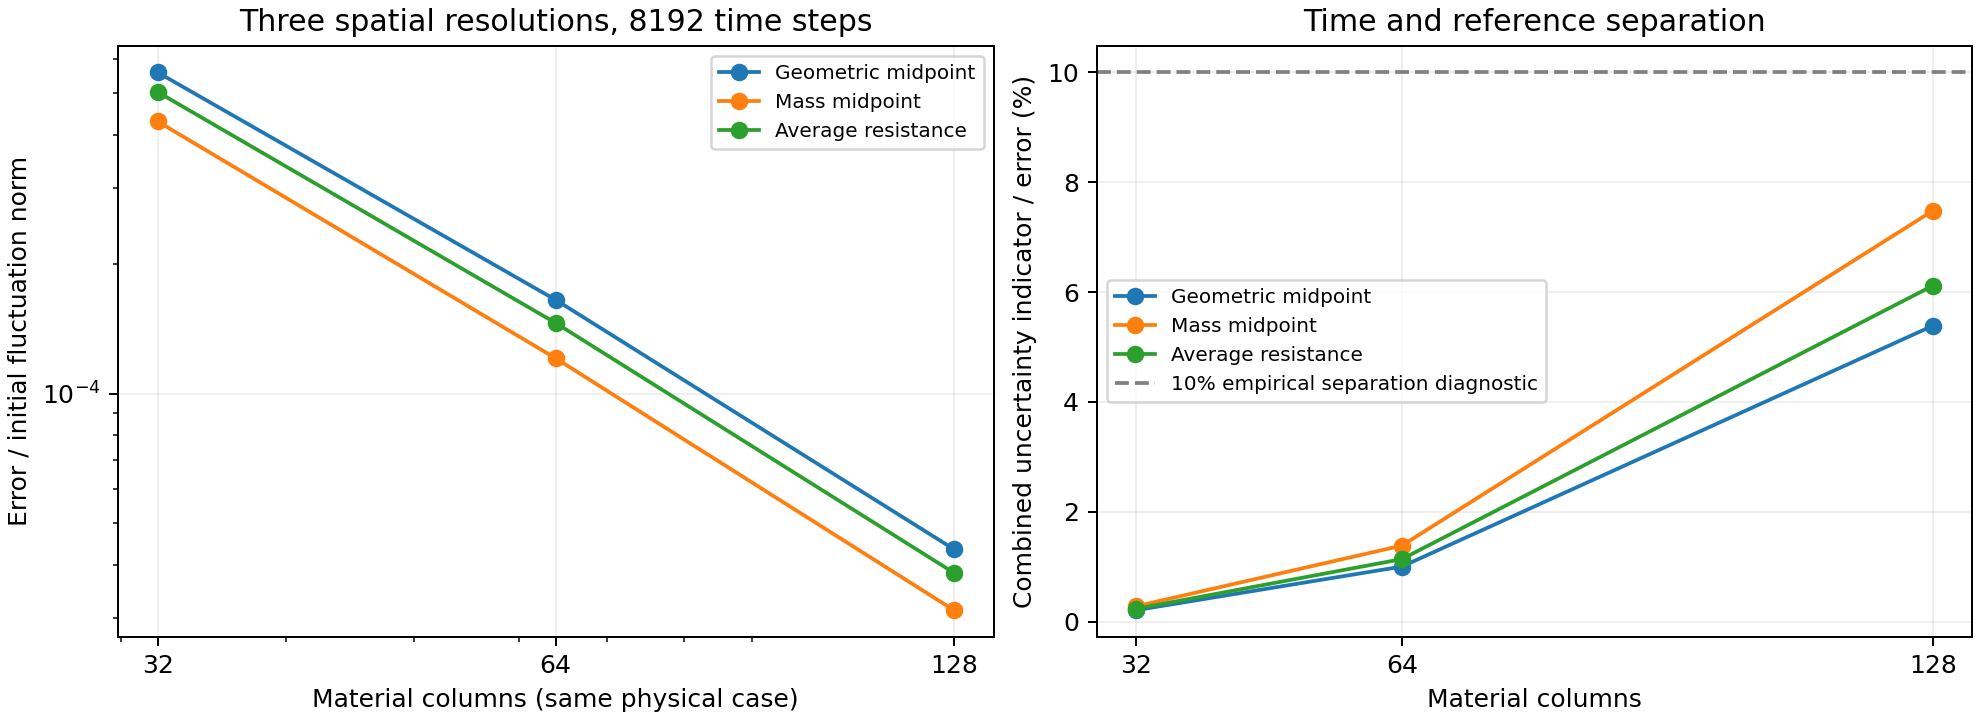
\includegraphics[width=0.9\textwidth,height=\textheight]{reports/project-20261107/figures/material-fv-space.png}
\caption{固定 Becker 问题的真实物质面 FV
空间细化；来源：runs/rebuild-stage3-space/spatial-convergence.png。}
\end{figure}

\begin{figure}
\centering
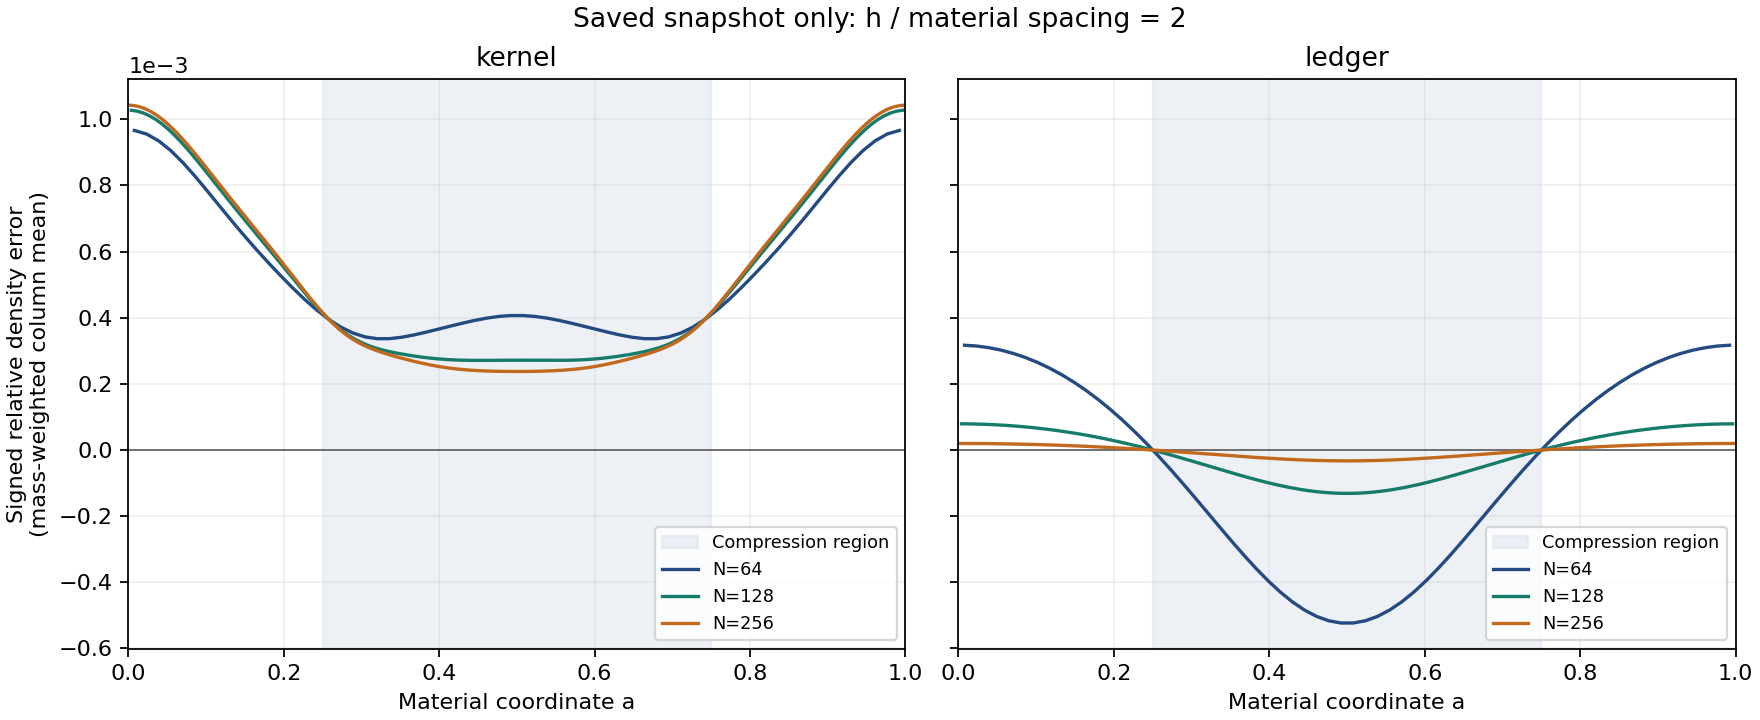
\includegraphics[width=0.95\textwidth,height=\textheight]{reports/project-20261107/figures/density-errors.png}
\caption{六个保存密度字段的有符号误差；来源：runs/reconnect-density-error-structure/signed-error-profiles-readable.png。}
\end{figure}

\subsection{来源和可追溯边界}\label{ux6765ux6e90ux548cux53efux8ffdux6eafux8fb9ux754c}

原始规范：\nolinkurl{docs/METHOD.md}、\nolinkurl{docs/CODEX_TASK.md}、\nolinkurl{docs/CODE_REVIEW.md}。主线回接、空间控制、同后端来源比较、联合证据及密度结构报告均由项目总览链接到原文件。原始交接的
782 个文件按独立清单校验；15
个附件保存在原工作区，本次下载包不包含它们。

旧 v080 未恢复，旧 246 项测试与早期原型数字没有被重新认证。当前 508
项是累计重建检查记录；本次代码交付只重跑 15
项既有小型检查，不增加科学完成度。Stage3 incomplete，fluid ORC 关闭。

\newpage

\section{代码导航与复现说明}\label{ux4ee3ux7801ux5bfcux822aux4e0eux590dux73b0ux8bf4ux660e}

2026-11-07。当前交付是研究代码整理，不冒用丢失的 ltnmix 0.8.0
版本。原算法文件和目录保持原样；新增统一入口负责导航、校验和有限的软件检查。

\subsection{目录职责}\label{ux76eeux5f55ux804cux8d23}

\begin{longtable}[]{@{}
  >{\raggedright\arraybackslash}p{(\columnwidth - 4\tabcolsep) * \real{0.3333}}
  >{\raggedright\arraybackslash}p{(\columnwidth - 4\tabcolsep) * \real{0.3333}}
  >{\raggedright\arraybackslash}p{(\columnwidth - 4\tabcolsep) * \real{0.3333}}@{}}
\toprule\noalign{}
\begin{minipage}[b]{\linewidth}\raggedright
路径
\end{minipage} & \begin{minipage}[b]{\linewidth}\raggedright
内容
\end{minipage} & \begin{minipage}[b]{\linewidth}\raggedright
使用方式
\end{minipage} \\
\midrule\noalign{}
\endhead
\bottomrule\noalign{}
\endlastfoot
\nolinkurl{docs/PROJECT_OVERVIEW.md} & 理论---代码---证据总览 &
首先阅读 \\
\nolinkurl{docs/NEXT_STEPS.md} & 当前工作计划 & 新实验尚未执行 \\
\nolinkurl{research/material_fv/} & 真物质面的一维 FV 基线 &
真实移动面是额外基准输入 \\
\nolinkurl{research/rebuild/} & Becker/接触重建与离散候选 &
各研究报告限定适用范围 \\
\nolinkurl{research/reconnect/} & 图层接口、点轨迹候选、参考与审计 &
不将全部脚本当一个成熟生产后端 \\
\nolinkurl{reference_baseline/}、\nolinkurl{prototypes/}、\nolinkurl{legacy_sources/}
& 782 个原文件所在的历史材料 & 保留字节，不整体导入旧运行脚本 \\
\nolinkurl{runs/} & 各轮保存证据 & 本次不新增上传；GitHub
只保留此前已有部分，源码 ZIP 不包含该目录 \\
\nolinkurl{tools/ltn_project.py} & 本次新增操作入口 & 小图检查、FV
检查、包完整性验证 \\
\nolinkurl{tools/build_project_report.py} & 总报告生成器 &
合并总览、理论附录、代码指南及下一步计划 \\
\nolinkurl{reports/project-20261107/} & 排版源、图、构建及检查记录 &
是整理交付，不是新的科学算例 \\
\nolinkurl{exports/} & PDF、代码 ZIP 与交付清单 & 下载及哈希核验 \\
\end{longtable}

没有搬迁或批量改名旧 Python
文件。研究脚本之间存在相对导入与封存源码哈希，目录整理通过导航和统一入口实现，避免改变既有数值行为。

\subsection{安装与快速检查}\label{ux5b89ux88c5ux4e0eux5febux901fux68c0ux67e5}

建议 Python 3.12。固定依赖见
\nolinkurl{backup/requirements-replay.txt}；它是已使用的研究环境版本清单，不代表旧
v080 环境恢复。

\begin{Shaded}
\begin{Highlighting}[]
\ExtensionTok{python3.12} \AttributeTok{{-}m}\NormalTok{ venv .venv}
\ExtensionTok{.venv/bin/python} \AttributeTok{{-}m}\NormalTok{ pip install }\AttributeTok{{-}r}\NormalTok{ backup/requirements{-}replay.txt}
\ExtensionTok{.venv/bin/python}\NormalTok{ tools/ltn\_project.py list}
\ExtensionTok{.venv/bin/python}\NormalTok{ tools/ltn\_project.py verify}
\ExtensionTok{.venv/bin/python}\NormalTok{ tools/ltn\_project.py checks }\AttributeTok{{-}{-}output}\NormalTok{ /tmp/ltn{-}checks{-}new}
\end{Highlighting}
\end{Shaded}

输出目录必须不存在。\nolinkurl{checks} 只运行两个已有软件检查组：小图链
10 项、一维 FV 5
项。它们验证导入、算子、时间顺序、守恒和受限解析控制，不运行 Becker
或大规模流体实验，不启用 ORC。既有 508 项记录不因重跑这 15 项而增加。

\nolinkurl{verify} 优先使用代码包内的
\nolinkurl{delivery-manifest.json}；完整 Git 检出则使用
\nolinkurl{backup/github-backup-manifest.json}。同时校验
\nolinkurl{backup/original-handoff-sha256.json} 的全部 782
个原文件。代码包的校验范围与 Git 精选恢复范围各自明确，不混称全量恢复。

\subsection{核心接口及边界}\label{ux6838ux5fc3ux63a5ux53e3ux53caux8fb9ux754c}

\begin{longtable}[]{@{}
  >{\raggedright\arraybackslash}p{(\columnwidth - 4\tabcolsep) * \real{0.3333}}
  >{\raggedright\arraybackslash}p{(\columnwidth - 4\tabcolsep) * \real{0.3333}}
  >{\raggedright\arraybackslash}p{(\columnwidth - 4\tabcolsep) * \real{0.3333}}@{}}
\toprule\noalign{}
\begin{minipage}[b]{\linewidth}\raggedright
对象
\end{minipage} & \begin{minipage}[b]{\linewidth}\raggedright
文件/函数
\end{minipage} & \begin{minipage}[b]{\linewidth}\raggedright
注意点
\end{minipage} \\
\midrule\noalign{}
\endhead
\bottomrule\noalign{}
\endlastfoot
轨迹、固定质量与图层传播 &
\nolinkurl{trajectory_chain.py}：\nolinkurl{TrajectorySamples}、\nolinkurl{propagate_supplied}
& 共享电导由调用者提供；位置本身不证明电导物理正确 \\
真实物质面基线 &
\nolinkurl{material_fv.py}：\nolinkurl{center_resistance}、\nolinkurl{step}、\nolinkurl{propagate}
& 单位横截面、一维、无通量端点、普通几何中点 \\
三种通量 & \nolinkurl{rebuild/experiment.py}：\nolinkurl{conductance} &
普通几何中心、质量中心、质量平均阻力是不同定义 \\
辅助面 &
\nolinkurl{periodic_voronoi_fv.py}：\nolinkurl{build_periodic_faces} &
不把 Voronoi 面积当成已知物质体积，不重算质量 \\
时间作用 &
\nolinkurl{voronoi_time_action.py}：\nolinkurl{operators}、\nolinkurl{exponential}、\nolinkurl{uniformization}
& 指数作用与独立递推；保持时间有序，不平均整个时间窗 \\
混合统计 & 同上：\nolinkurl{metrics}、\nolinkurl{dissipation} &
\nolinkurl{variance} 为未除总质量的平方和；H
使用比值，绝对耗散须核对因子 \\
密度来源 &
\nolinkurl{t1_density_sources.py}、\nolinkurl{compression_density_sources.py}
& 原 kernel 和固定邻居环 ledger 均保持原定义；无 F
拟合、裁剪或离散重归一化 \\
\end{longtable}

\subsection{如何复核一个旧结果}\label{ux5982ux4f55ux590dux6838ux4e00ux4e2aux65e7ux7ed3ux679c}

先读该案例的报告、配置、源码锁及哈希，再运行对应只读审计。不要直接执行名称含
\nolinkurl{study}、\nolinkurl{deliver}、\nolinkurl{package}
的脚本来``快速测试''：有的依赖未打包的历史数据，有的会进行长计算或生成交付文件。

例如完整本地工作区包含所需来源时，可按报告中的命令核验
\nolinkurl{runs/reconnect-density-error-structure/}。本次 GitHub
更新没有上传这组新数据，代码 ZIP 也不含
\nolinkurl{runs/}，所以不能声称只靠小包或当前远端就能重算所有保存物理结果。缺失输入应明确报告，不能伪造或更换。

\subsection{重建 PDF}\label{ux91cdux5efa-pdf}

需要 Pandoc、XeLaTeX、Noto CJK 字体和常用 LaTeX 包，数值依赖不参与排版。

\begin{Shaded}
\begin{Highlighting}[]
\ExtensionTok{python}\NormalTok{ tools/build\_project\_report.py}
\end{Highlighting}
\end{Shaded}

图表使用随报告保存的既有结果图；生成器不运行物理求解器。排版源和 PDF
的文件哈希记录在交付清单。原始 README、METHOD、CODEX\_TASK 及 PHASE
文档不为新交付而改写。

\newpage

\section{下一步工作计划：先完成平滑流闭环，再推进接触与激波}\label{ux4e0bux4e00ux6b65ux5de5ux4f5cux8ba1ux5212ux5148ux5b8cux6210ux5e73ux6ed1ux6d41ux95edux73afux518dux63a8ux8fdbux63a5ux89e6ux4e0eux6fc0ux6ce2}

2026-11-07。本计划承接项目总览和保存结果。此次授权范围是完整
PDF、代码整理、GitHub 更新和规划；下列新物理实验尚未执行。Stage3
incomplete，fluid ORC 关闭。

\subsection{目标与推进方式}\label{ux76eeux6807ux4e0eux63a8ux8fdbux65b9ux5f0f}

要完成的主张是：在明确的输入、边界和本构范围内，固定质量的局部正交换能够准确预测物质平均浓度及其掺混，并且误差可与时间离散、参考解和密度来源区分。

每项工作一次交付``问题、必要实现、一次实验、核验、结论''，不再把契约编写、预算说明和审计次数各自当成一轮科学进展。只在新结果确实无法判别且存在明确可消除的误差来源时，讨论补充计算。旧失败和未决不改判。

\subsection{P0：本次完成交付与恢复入口}\label{p0ux672cux6b21ux5b8cux6210ux4ea4ux4ed8ux4e0eux6062ux590dux5165ux53e3}

\begin{itemize}
\tightlist
\item
  总报告同时提供 Markdown、排版 PDF 和可重建排版源码。
\item
  新增代码地图、统一检查入口和小型代码
  ZIP；保留历史源码路径，以免破坏封存哈希。
\item
  GitHub main 保留已有远端历史，仅新增研究代码、文档和本次
  PDF/源码包；本次不新增运行数据，历史大 ZIP 留在本地。
\item
  精选恢复与全量工作区区分。15 个原附件、全部历史大运行和旧 v080
  不宣称已经通过本次 GitHub 更新恢复。
\end{itemize}

完成标志：可下载 PDF/代码包；从独立目录解包后能校验清单并运行小图与 FV
既有检查；远端提交经读取确认。它不是 Stage3 的新增物理证据。初次包含约
1.2 GB
新对象及运行结果的推送被自动审批拒绝，因未获明确公开这些数据的授权；实际更新收紧为本次所需报告和代码。

\subsection{P1：下一项科学工作------一个平滑流的 ledger
瞬态空间对照}\label{p1ux4e0bux4e00ux9879ux79d1ux5b66ux5de5ux4f5cux4e00ux4e2aux5e73ux6ed1ux6d41ux7684-ledger-ux77acux6001ux7a7aux95f4ux5bf9ux7167}

\textbf{问题：单个光滑密度快照中 ledger
的误差下降，是否能转化为同一交换后端下、整个时间窗的浓度与 H
空间一致性？} 当前快照结论不能回答它，N64 单例也不能回答它。

\begin{longtable}[]{@{}
  >{\raggedright\arraybackslash}p{(\columnwidth - 2\tabcolsep) * \real{0.5000}}
  >{\raggedright\arraybackslash}p{(\columnwidth - 2\tabcolsep) * \real{0.5000}}@{}}
\toprule\noalign{}
\begin{minipage}[b]{\linewidth}\raggedright
项目
\end{minipage} & \begin{minipage}[b]{\linewidth}\raggedright
预定范围
\end{minipage} \\
\midrule\noalign{}
\endhead
\bottomrule\noalign{}
\endlastfoot
物理问题 & 复用已有非线性周期压缩，D=.02、T=.05；只看已登记 t=.025 和
.05 \\
空间资料 & N64/128/256 的原轨迹、物质质量、c0、父子投影和 oracle 参考 \\
比较对象 & 固定环 ledger 与
oracle；同一普通中心阻力辅助面后端，保持密度语义和单位 \\
可复用项 & 全部已保存 oracle 路径、参考、N64 ledger
路径和可核对的原几何 \\
预计缺项上限 & 若来源核对成立，仅 N128/256 各 K8/16/32 的 ledger
路径及其必要系数和独立核验；最多六条实际路径，不新增几何或参考 PDE \\
时间证据 & N64 复用已有 K16/32/64；细两档以 K8/16/32
检查三档时间差，空间主比较共同使用 K32；各组判定分别报告 \\
判别 & 原生浓度、共同物质观察浓度和 H
分列；保留原时间/参考/投影/数值正项，不能用共同投影隐藏细尺度误差 \\
停止 &
原资料缺失或时刻/质量不匹配时停在明确缺项；误差不降或未分辨时报告并停止，不自动增
N、K 或参考 \\
\end{longtable}

上表是规划上限，尚未证明所有路径和参考都已满足可复用条件，不能据此宣称``只差六次运行''或保证通过。开始时在同一任务内完成来源核对，再决定能否直接实施。

原 fixed-ratio kernel 案例已经失败并触发停止；P1 不重跑它，不用调
h、归一化或拟合来追求排名。固定旧带宽卷积诊断只保留为备选机制研究，不自动重启。P1
只补 ledger 的有限范围证据，不能单独关闭三密度来源的 Stage3 要求。

\subsection{P2：独立接触间断的密度来源判别}\label{p2ux72ecux7acbux63a5ux89e6ux95f4ux65adux7684ux5bc6ux5ea6ux6765ux6e90ux5224ux522b}

P1 给出可解释结论后，再选择已经有 oracle
三空间档参考的静态接触问题。先在一个原分辨率上比较 oracle、原 kernel
和无 F 修正 ledger，所有来源共用 m、c0、D、边界与交换后端。

必须分别检查单侧点密度、跨界物质单元平均及实际共享扩散通量；不在接触面用零质量通量相除推密度比。候选失败时定位是密度目标、几何闭合还是交换规则失效，并限制适用范围；不靠平滑抹掉物理间断。

只有单例差异超过时间与参考不确定度，且结果支持进一步验证时，才补原规范要求的空间档。此时仍不做参数全矩阵；若单例已否定当前候选，保存反例即可。

\subsection{P3：回到 Becker
激波，分开两类缺口}\label{p3ux56deux5230-becker-ux6fc0ux6ce2ux5206ux5f00ux4e24ux7c7bux7f3aux53e3}

\begin{enumerate}
\def\labelenumi{\arabic{enumi}.}
\tightlist
\item
  \textbf{来源比较}：优先复用 δ=.08、D=.02、T=.1、32 个物质列的现成
  oracle 和参考，开展一个同后端来源判别。保留所有旧空间和 H
  时间未决，不将新来源结果回填旧行。
\item
  \textbf{层厚度控制}：δ=.04 已有 N32 对照但没有对应三空间档，H
  时间未分辨。先说明已有预算允许识别什么，再决定是否补最小缺项。不得用简单再加
  K 或再细化参考来保证通过；当前预算已有相应限制。
\end{enumerate}

两项分别回答``密度来源在激波中是否可用''和``物理层变薄时离散如何变化''，不能混在一次扫描里。平面激波关系不外推曲面非定常激波。

\subsection{P4：一次正式验收汇总，而不是继续加项目}\label{p4ux4e00ux6b21ux6b63ux5f0fux9a8cux6536ux6c47ux603bux800cux4e0dux662fux7ee7ux7eedux52a0ux9879ux76ee}

将原 METHOD/CODEX\_TASK
每条要求对到最终采用的后端、边界、来源和实测误差。已有 T1--T3、接触
oracle、Becker 共同 K32 成果直接引用，不重复计算。

\begin{itemize}
\tightlist
\item
  保守性、正性等代数检查与 PDE 精度各自列出。
\item
  各项原有要求、失败与未决公开；不得事后删除不利项目，或把``ledger
  必须优于 oracle''追加为条件。
\item
  新候选不能借其他后端的通过记录获得通用资格；默认方案与实验对照明确标注。
\item
  如果原声明范围仍有实质缺口，Stage3 保持
  incomplete。若建议缩小方法范围，应明确这是范围调整，不能冒称原范围完整通过。
\item
  完成相应流体物理验收后，才进入动态 ORC 与 H
  联合解释。DNS、T5/T6、复杂二维应用另列后续任务。
\end{itemize}

目前不能承诺 Stage3 的通过日期。可承诺的是：下一次科学推进只回答 P1
的一个问题，并以有效证据、失败或明确未决结束；不会用检查数量或报告页数代替完成程度。

\end{document}
